\chapter{Detailed results of VGG16\_block5\_pool\_max with Cosine distance}

\label{chapter:ResultsVGG16Block5PoolMax}

% ----------------

In this appendix, we present the detailed results of the benchmark for \textit{VGG16\_block5\_pool\_max} with Cosine distance.

\begin{figure*}
	\centering
	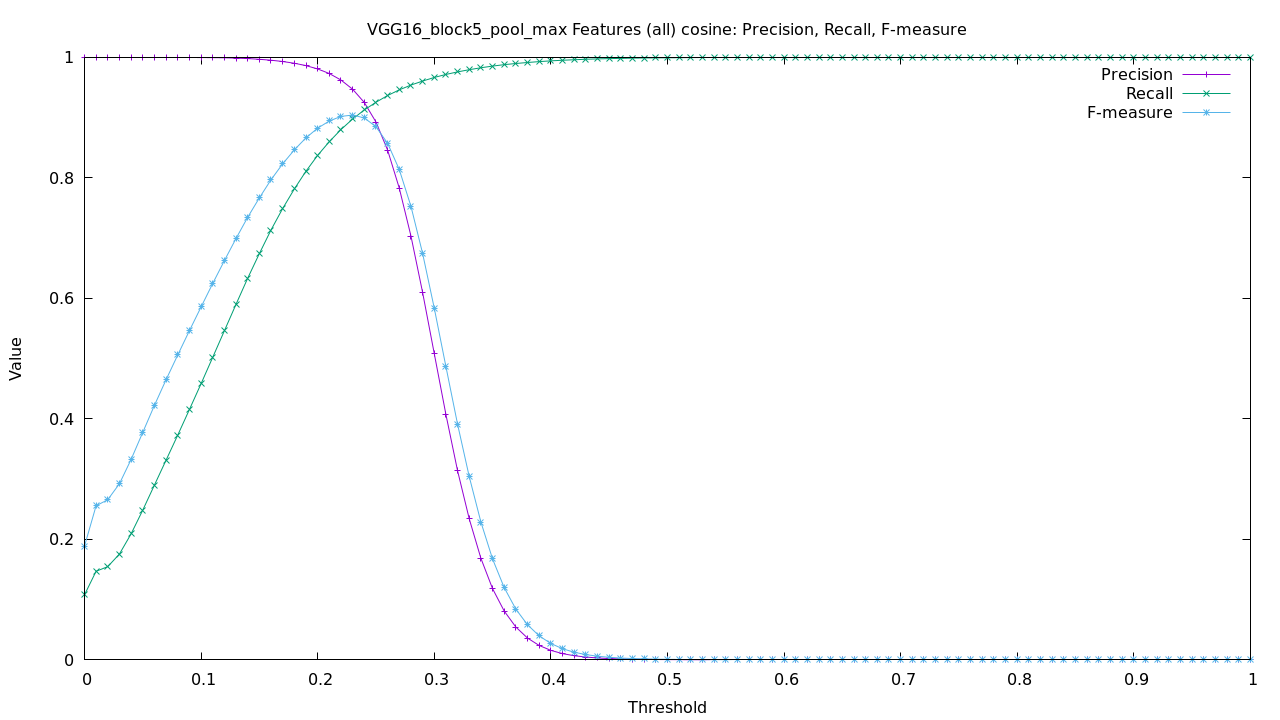
\includegraphics[width=\textwidth]{img/benchmark_VGG16_block5_pool_max_cosine_all.png}
	\caption{Precision, recall, Fmeasure, curves of \textit{VGG16\_block5\_pool\_max} search results with all modifications according to different radius (threshold).}
	\label{fig:benchmark_VGG16_block5_pool_max_cosine_all}
\end{figure*}

\begin{figure*}
	\centering
	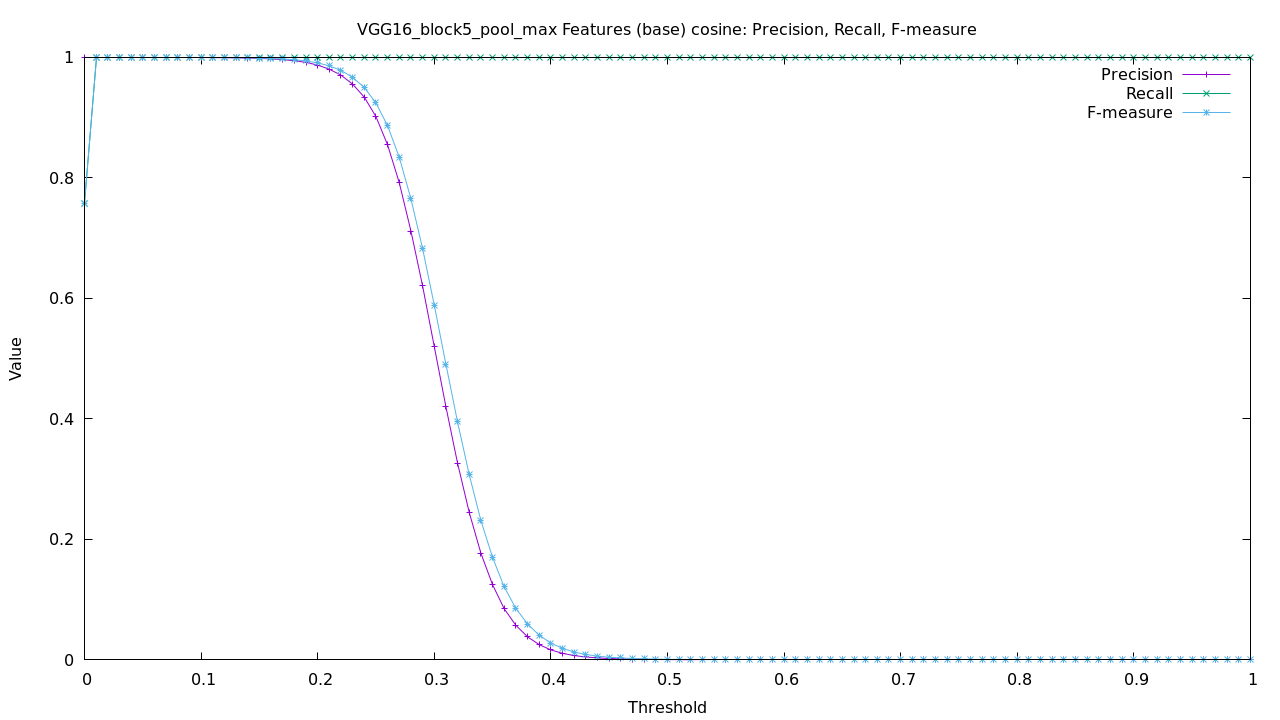
\includegraphics[width=\textwidth]{img/benchmark_VGG16_block5_pool_max_cosine_base.png}
	\caption{Precision, recall, Fmeasure, curves of \textit{VGG16\_block5\_pool\_max} search results with no modification according to different radius (threshold).}
	\label{fig:benchmark_VGG16_block5_pool_max_cosine_base}
\end{figure*}

\begin{figure*}
	\centering
	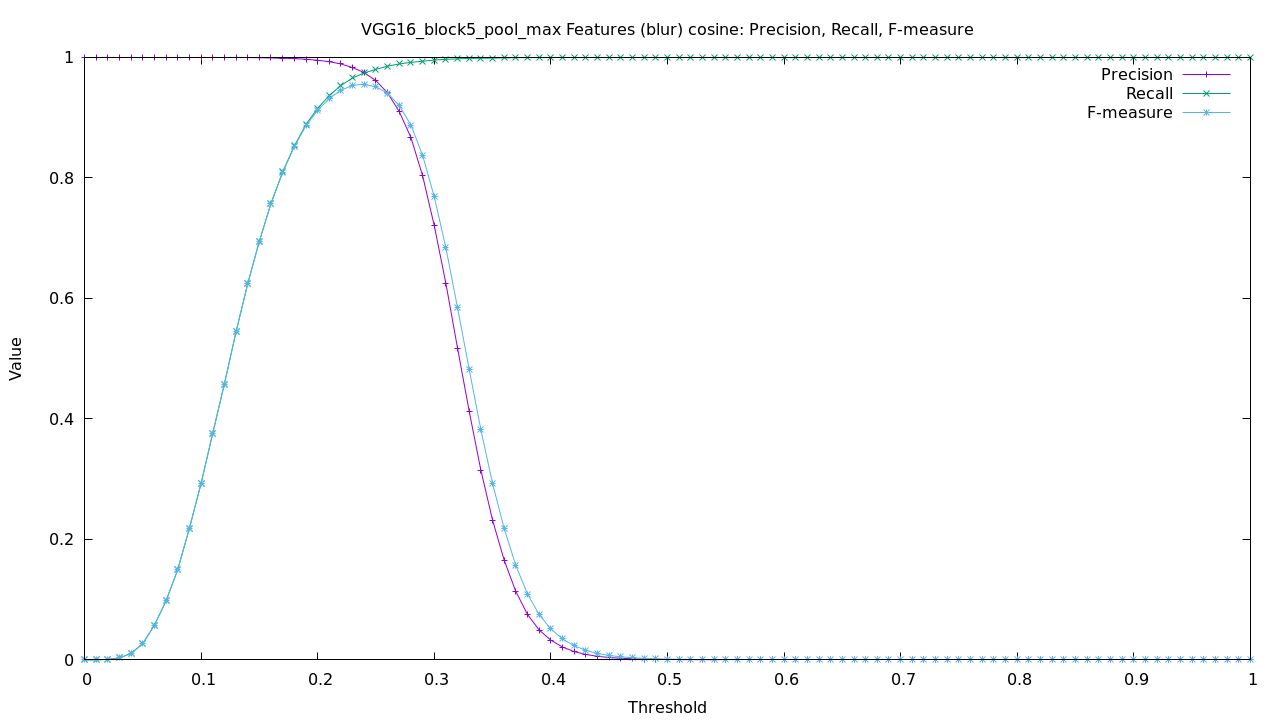
\includegraphics[width=\textwidth]{img/benchmark_VGG16_block5_pool_max_cosine_blur.png}
	\caption{Precision, recall, Fmeasure, curves of \textit{VGG16\_block5\_pool\_max} search results only with Gaussian blur ($r=4$, $\Sigma=2$) according to different radius (threshold).}
	\label{fig:benchmark_VGG16_block5_pool_max_cosine_blur}
\end{figure*}

\begin{figure*}
	\centering
	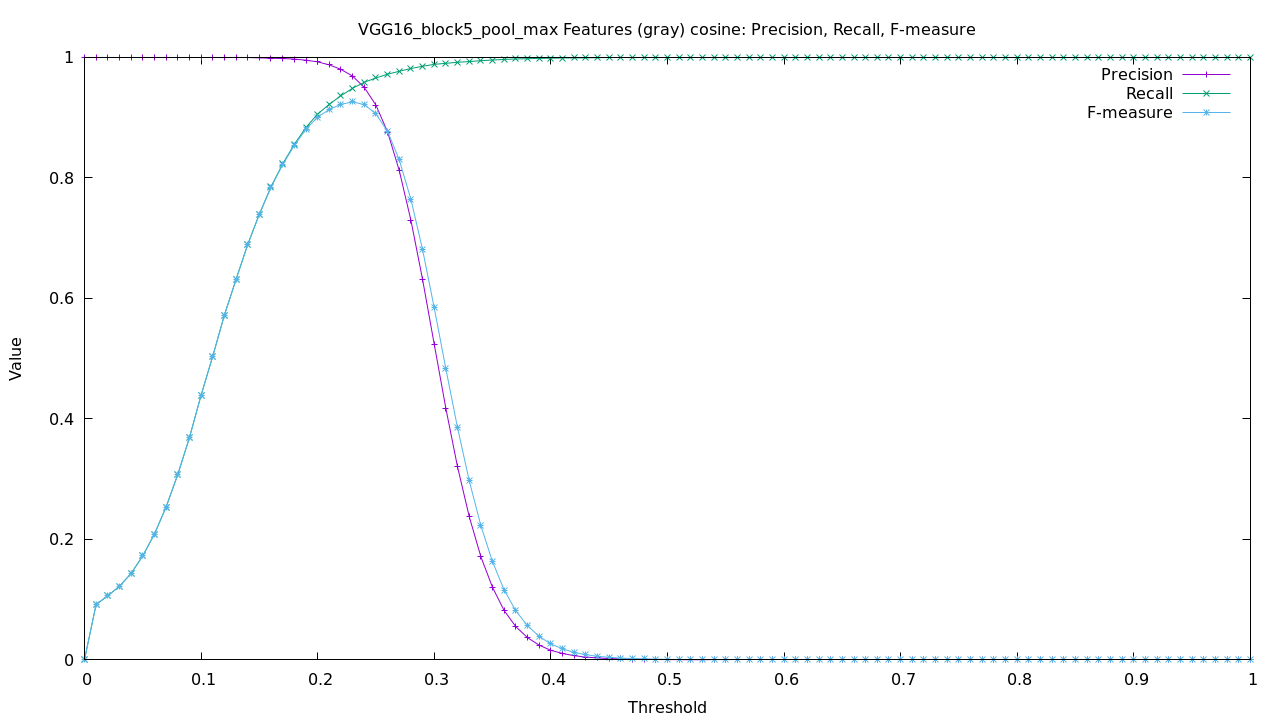
\includegraphics[width=\textwidth]{img/benchmark_VGG16_block5_pool_max_cosine_gray.png}
	\caption{Precision, recall, Fmeasure, curves of \textit{VGG16\_block5\_pool\_max} search results only with grayscale filter according to different radius (threshold).}
	\label{fig:benchmark_VGG16_block5_pool_max_cosine_gray}
\end{figure*}

\begin{figure*}
	\centering
	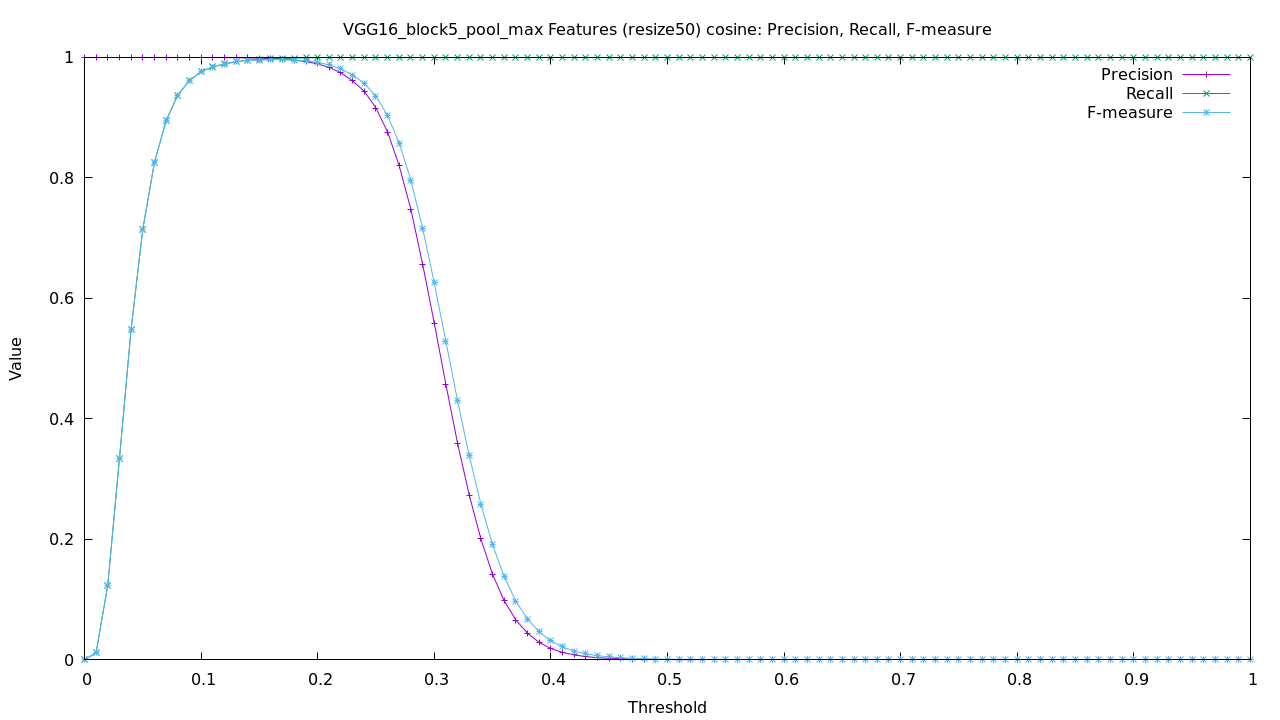
\includegraphics[width=\textwidth]{img/benchmark_VGG16_block5_pool_max_cosine_resize50.png}
	\caption{Precision, recall, Fmeasure, curves of \textit{VGG16\_block5\_pool\_max} search results only with resize to half size according to different radius (threshold).}
	\label{fig:benchmark_VGG16_block5_pool_max_cosine_resize50}
\end{figure*}

\begin{figure*}
	\centering
	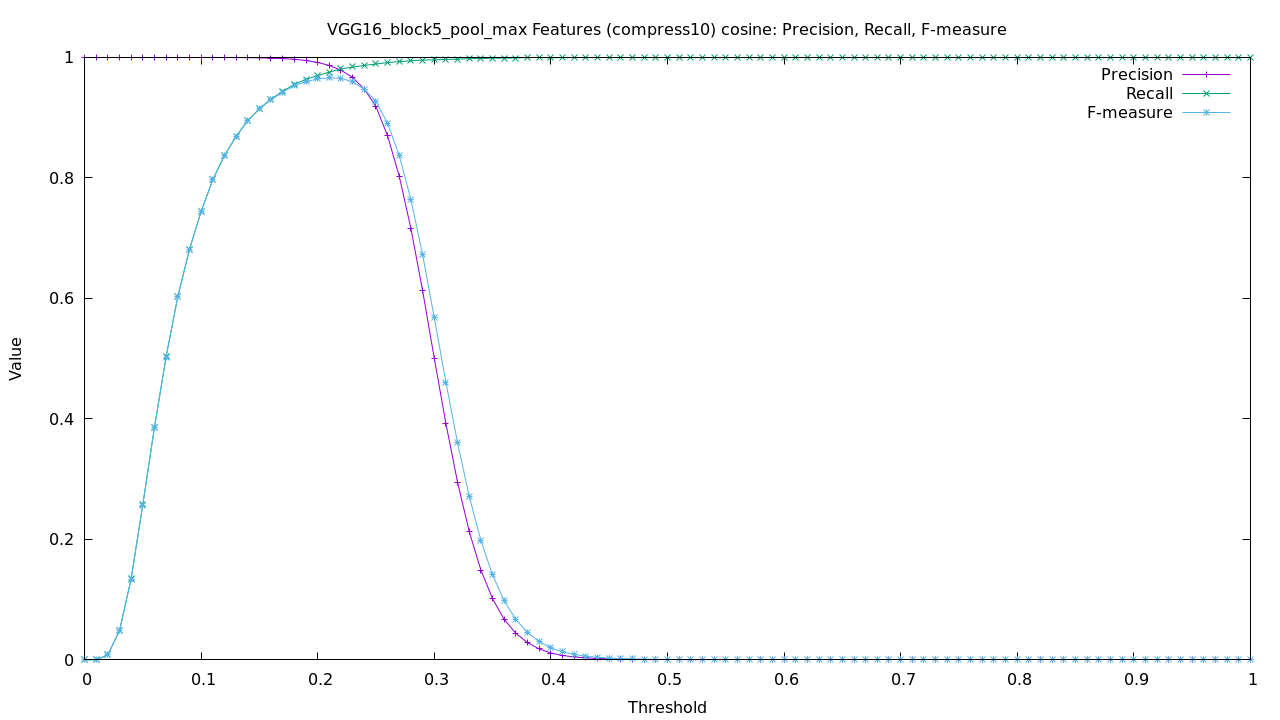
\includegraphics[width=\textwidth]{img/benchmark_VGG16_block5_pool_max_cosine_compress10.png}
	\caption{Precision, recall, Fmeasure, curves of \textit{VGG16\_block5\_pool\_max} search results only with JPEG compression (quality 10\%) according to different radius (threshold).}
	\label{fig:benchmark_VGG16_block5_pool_max_cosine_compress10}
\end{figure*}

\begin{figure*}
	\centering
	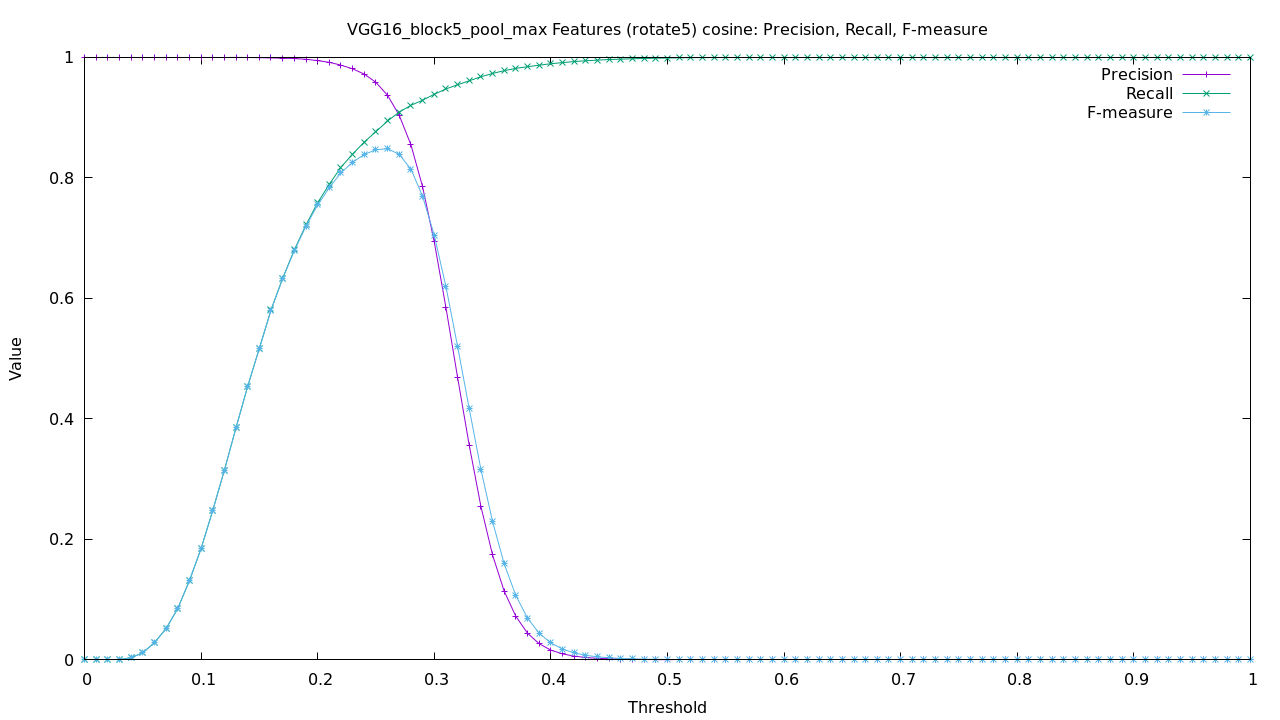
\includegraphics[width=\textwidth]{img/benchmark_VGG16_block5_pool_max_cosine_rotate5.png}
	\caption{Precision, recall, Fmeasure, curves of \textit{VGG16\_block5\_pool\_max} search results only with clockwise rotation by 5 degrees according to different radius (threshold).}
	\label{fig:benchmark_VGG16_block5_pool_max_cosine_rotate5}
\end{figure*}

\begin{figure*}
	\centering
	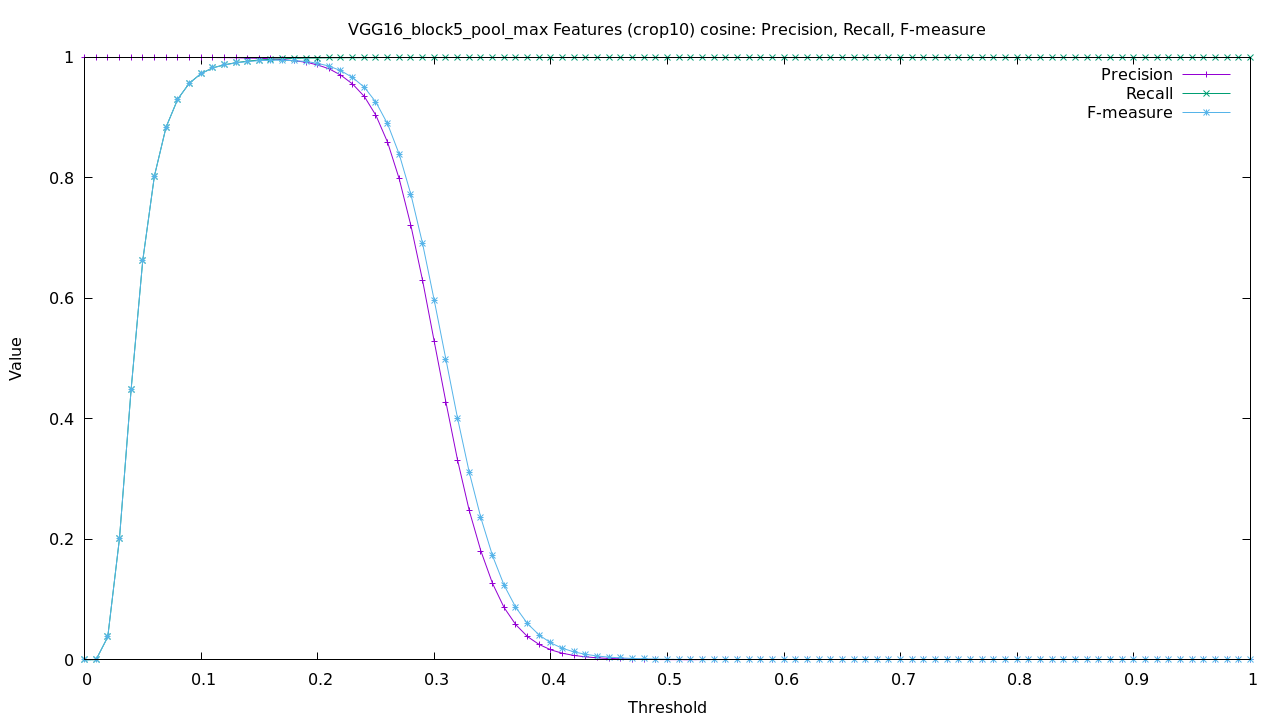
\includegraphics[width=\textwidth]{img/benchmark_VGG16_block5_pool_max_cosine_crop10.png}
	\caption{Precision, recall, Fmeasure, curves of \textit{VGG16\_block5\_pool\_max} search results only with cropping by 10\% at the right side of the image according to different radius (threshold).}
	\label{fig:benchmark_VGG16_block5_pool_max_cosine_crop10}
\end{figure*}